\section{A rival's options: the completing deed}
\label{sec:rival}

\subsection{What happens to an offer that completes the proposer's group}
The agents answered \fact{o.census.responses.n} offers with \fact{o.census.responses.accept} acceptances, \fact{o.census.responses.counter} counters and \fact{o.census.responses.reject} rejections. Each system accepted between \fact{o.census.by-recipient.Gemini.accept} and \fact{o.census.by-recipient.Sol.accept} offers. They differ in how they disagree: Sol and Opus countered \fact{o.census.by-recipient.Sol.counter} and \fact{o.census.by-recipient.Opus.counter} times, and Gemini and Grok rejected \fact{o.census.by-recipient.Gemini.reject} and \fact{o.census.by-recipient.Grok.reject}.

A deed that would complete the proposer's color group is the clearest case of a move that opens something for a rival, because only a complete group can be built on. Table~\ref{tab:opening} gives every opening offer by form and by who would complete a group. We compare opening offers because later offers are shaped by what both sides have already refused (Appendix~\ref{app:offers}).

\begin{table}[t]\centering\small
\TableOpening
\caption{All \fact{o.census.opening} acceptance-legal opening offers. A swap moves deeds both ways. A cash bid offers only cash for deeds. A sale offer offers only deeds for cash. ``Other'' holds the remaining forms. Completion is evaluated on ownership after the proposed transfer. Empty cells are omitted: a cash bid cannot complete the recipient's group and a sale offer cannot complete the proposer's.}
\label{tab:opening}\end{table}

An opening swap or cash bid that would complete only the proposer's group was accepted \fact{x.po.accept} times in \fact{x.po.n}. Recipients rejected \fact{x.po.reject} and countered \fact{x.po.counter}. The same two forms, when they completed nobody's group, were accepted \fact{x.nei.accept} times in \fact{x.nei.n}.

\subsection{Swaps are refused and cash bids are priced}
The response depends on what the proposer puts on the table. Recipients rejected \fact{o.headline-cells.swap-proposer-only.reject} of \fact{o.headline-cells.swap-proposer-only.n} swaps that completed only the proposer (\fact{x.swpo.rej.pct}\%) and \fact{o.headline-cells.swap-neither.reject} of \fact{o.headline-cells.swap-neither.n} that completed nobody (\fact{x.swn.rej.pct}\%), a gap of \fact{o.sensitivity.swap-gap.point-pp} percentage points. Swaps that completed both sides fall between, at \fact{o.headline-cells.swap-both.reject} of \fact{o.headline-cells.swap-both.n}. For cash bids the two rates are \fact{o.headline-cells.cash-bid-proposer-only.reject} of \fact{o.headline-cells.cash-bid-proposer-only.n} and \fact{o.headline-cells.cash-bid-neither.reject} of \fact{o.headline-cells.cash-bid-neither.n}, a difference of \fact{o.sensitivity.cash-bid-gap.point-pp} points (Figure~\ref{fig:offers}A).

\begin{figure}[t]\centering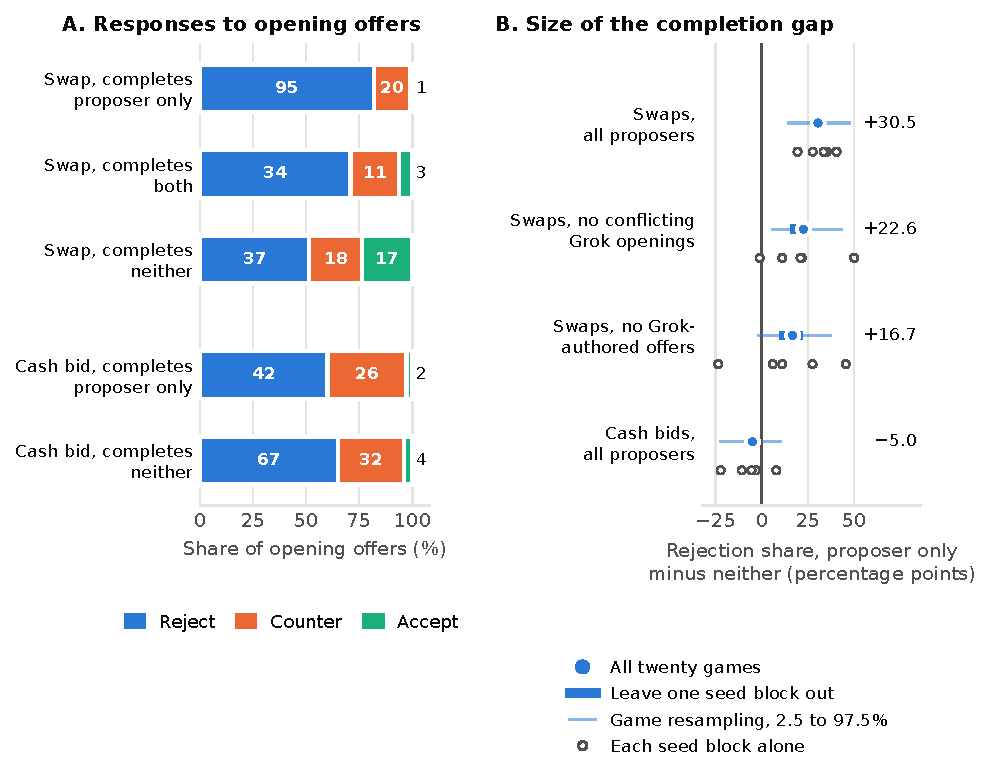
\includegraphics[width=\linewidth]{offer_responses.pdf}
\caption{Opening offers. A: responses by form and completion, as shares with counts printed. B: the rejection share for offers completing only the proposer minus the share for offers completing nobody. The dot uses all twenty games. The thick bar is the range when one seed block is left out. The thin line spans the middle 95\% of 20,000 resamples of the twenty games. Open circles are the five seed blocks taken alone. These describe how one cohort's contrast depends on its games. They are not intervals for new games.}
\label{fig:offers}\end{figure}

The swap gap holds in direction for every recipient, every proposer and every seed block (Table~\ref{tab:strata}). Its size depends on who wrote the comparison offers. Grok wrote \fact{o.composition.swap-neither-by-grok} of the \fact{o.headline-cells.swap-neither.n} swaps that completed nobody and \fact{o.composition.swap-neither-accepted-by-grok} of the \fact{o.composition.swap-neither-accepted} that were accepted, and \fact{o.composition.swap-neither-accepted-conflict-openings} of those acceptances answered openings whose text named a different action. Without the conflicting openings the gap is \fact{o.sensitivity.swap-gap-without-conflict-openings.point-pp} points. Without any Grok-authored swap it is \fact{o.sensitivity.swap-gap-without-grok-authors.point-pp} points (\fact{o.composition.without-grok-authors.swap-proposer-only.0} of \fact{o.composition.without-grok-authors.swap-proposer-only.1} against \fact{o.composition.without-grok-authors.swap-neither.0} of \fact{o.composition.without-grok-authors.swap-neither.1}). Weighting the within-proposer gaps by three choices of proposer mix gives \fact{o.composition.standardized-swap-gap-pp.weights-proposer-only-cell} to \fact{o.composition.standardized-swap-gap-pp.weights-neither-cell} points. Removing offers shows how the count depends on them, not what the other agents would have done in games without them. Table~\ref{tab:sens} gives the ranges under each version. Leaving out any one seed block keeps the gap positive in every version. In the version without Grok's offers both resampling ranges reach below zero, and in both reduced versions one seed block taken alone is negative.

\begin{table}[t]\centering\small
\TableStrata
\caption{Rejected over received, opening offers, by proposer and by recipient. Within every recipient the swap gap is positive (\fact{x.rec.Opus.swgap} to \fact{x.rec.Sol.swgap} points) and the cash-bid gap is between \fact{x.rec.Opus.cbgap} and \fact{x.rec.Sol.cbgap} points. Opus wrote \fact{o.composition.cash-bids-in-headline-cells-by-opus} of the \fact{o.composition.cash-bids-in-headline-cells} cash bids.}
\label{tab:strata}\end{table}

\begin{table}[t]\centering\footnotesize
\TableSensitivity
\caption{How the selected contrasts depend on the games included. Values are percentage points. ``Seed-block resampling'' is the 2.5th to 97.5th percentile over all 3,125 ordered resamples of five blocks. ``Game resampling'' is the same percentiles over 20,000 resamples of twenty games. The contrasts were chosen after inspecting these games, and the games share seeds and one roster, so the ranges describe this cohort and are not confidence intervals.}
\label{tab:sens}\end{table}

For cash bids the pooled difference is negative, the difference within each recipient lies between \fact{x.rec.Opus.cbgap} and \fact{x.rec.Sol.cbgap} points, and both resampling ranges include zero. These records show no completion gap for cash bids. They do not show that one is absent.

What differs is the kind of reply. Recipients countered \fact{o.headline-cells.cash-bid-proposer-only.counter} of \fact{o.headline-cells.cash-bid-proposer-only.n} completing cash bids (\fact{x.cbpo.ctr.pct}\%) and \fact{o.headline-cells.swap-proposer-only.counter} of \fact{o.headline-cells.swap-proposer-only.n} completing swaps (\fact{x.swpo.ctr.pct}\%), a difference with the same sign in all five seed blocks. In \fact{o.counters.opening-cash-bid-proposer-only.same-bundle-more-cash} of the \fact{o.counters.opening-cash-bid-proposer-only.counters} cash-bid counters the recipient kept the deeds as proposed and asked for more money.

\subsection{What the refusals say, and how the systems differ}
The stated reasons do not separate the two forms. A pattern match finds completion or blocking language in \fact{o.keyword-screen.rejections.swap-proposer-only.completion-terms} of the \fact{o.keyword-screen.rejections.swap-proposer-only.n} rejections of completing swaps and in all \fact{o.keyword-screen.rejections.cash-bid-proposer-only.n} rejections of completing cash bids, and building language in \fact{o.keyword-screen.rejections.swap-proposer-only.building-terms} and \fact{o.keyword-screen.rejections.cash-bid-proposer-only.building-terms}.

\begin{table}[t]\centering\small
\TableStyles
\caption{Responses to the \fact{x.po.n} opening swaps and cash bids that would complete only the proposer's group, by recipient. The right-hand columns are regular-expression counts over the public message and applied note of each rejection: building terms (house, hotel, build, develop), reciprocity terms (``in return'', ``for me as well'' and similar) and commitment terms (``never'', ``not for sale'', ``do not counter''). Opus answered \fact{x.opus.recovery.trade.responses} of its \fact{o.census.by-recipient.Opus.n} trade responses through action-only recovery, without a note.}
\label{tab:styles}\end{table}

The systems refuse in recognizably different ways (Table~\ref{tab:styles}). Gemini rejected \fact{x.style.Gemini.rej.pct}\% of these openings and often stated a rule, as in G4: \InlineQuote{in-g4-d72-rule} Grok rejected \fact{x.style.Grok.rej.pct}\% and paired dollar estimates of the rival's building cash with a commitment not to bargain, as in G1: \InlineQuote{in-g1-d122-commit} Sol rejected \fact{x.style.Sol.rej.pct}\% and countered the rest. Opus countered \fact{o.refusal-wording.responses-by-recipient-proposer-only-openings.Opus.counter} of \fact{o.refusal-wording.responses-by-recipient-proposer-only-openings.Opus.n}.

An earlier coding of stated reasons in this project covers a different population. Two model-assisted readings agreed that \fact{o.semantic-codes.agreed-rival-consequence} of \fact{o.semantic-codes.coded-rows} rejections named a consequence for the rival. All \fact{o.semantic-codes.coded-rows} are rejections of offers that would complete the recipient's own group, so none falls in the cells compared above. They show that agents state rival concern even when refusing their own monopoly, and they cannot explain why swaps and cash bids are treated differently. Incident 2 is one of those refusals.

\IncidentTitle{g15}{Refusing one's own monopoly to deny a rival's}
At G15 turn 63 Sol holds \$730 and two greens. Grok holds \$333, the third green and Ventnor, the yellow Sol lacks. One turn earlier Opus had told the table, \InlineQuote{in-g15-d166-appeal}. Sol offers both greens for Ventnor and \$100, which would complete a group for each side. Grok refuses, and its note compares what each could then build:
\TranscriptQuote{g15-d169-note}
The cash figures are right. A first row of green houses does cost \$600, although a single \$200 house would have been legal. Sol drops the cash request and adds Kentucky, is refused again, and then restates the comparison in Grok's terms:
\TranscriptQuote{g15-d174-sweetener}
\TranscriptQuote{g15-d175-refusal}
All three offers fail, and Gemini refuses a different Sol offer on the same turn. Eighteen turns later Grok goes bankrupt to Gemini, which inherits its deeds and wins. Sol never completes yellow or green. Whether accepting would have served Grok better is not known.
\IncidentSource{G15 d166 to d176, standard responses. The Opus appeal is in Grok's prompt at d169. Each public message appears in the counterparty's next prompt.}

\subsection{Does refusal follow the size of the rival's opportunity?}
Grok's note in G15 reasons about amounts: how much the rival would hold and how many houses that buys. If refusals in general followed that reasoning, they would be more common when the proposer would keep more building cash. They are not. Among completing swaps, recipients rejected \fact{o.rival-capacity.swap-proposer-only.1-2.reject} of \fact{o.rival-capacity.swap-proposer-only.1-2.n} when the proposer could afford one or two houses after the trade, \fact{o.rival-capacity.swap-proposer-only.3-5.reject} of \fact{o.rival-capacity.swap-proposer-only.3-5.n} for three to five, and \fact{o.rival-capacity.swap-proposer-only.6+.reject} of \fact{o.rival-capacity.swap-proposer-only.6+.n} for six or more. When the proposer could afford none, they rejected \fact{o.rival-capacity.swap-proposer-only.0.reject} of \fact{o.rival-capacity.swap-proposer-only.0.n}, too few to read. Completing cash bids show no order either (Appendix~\ref{app:offers}). The measure ignores what the proposer could still mortgage, so it is coarse.

A crude check speaks against the simplest alternative, that completing swaps are refused because they pay badly. At board list prices the completing swaps offered the recipient more, a median of \$\fact{o.list-value.swap-proposer-only.median-net-list-value-to-recipient} against \$\fact{o.list-value.swap-neither.median-net-list-value-to-recipient}. Among swaps that favored the recipient at list price, \fact{o.list-value.swap-proposer-only.favourable-to-recipient.0} of \fact{o.list-value.swap-proposer-only.favourable-to-recipient.1} completing ones were rejected and \fact{o.list-value.swap-neither.favourable-to-recipient.0} of \fact{o.list-value.swap-neither.favourable-to-recipient.1} of the others. List price leaves out mortgages, group value and the value of blocking, so this narrows the alternative without removing it. The stated amounts are also not always right.

\IncidentTitle{g2}{A price set on the buyer's building budget, with the wrong house count}
At G2 turn 44 Grok, which owns no yellow, bids \$200 for Sol's Marvin Gardens, and Sol asks \$450. On turn 45 Opus, which owns the other two yellows and has \$845, bids \$325 for the same deed. Sol asks \$650 and records why:
\TranscriptQuote{g2-d124-note}
Both subtractions are right. The house count is wrong. Yellow houses cost \$150, so \$520 buys three. Opus raises to \$450 and says \InlineQuote{in-g2-d127-final} Its note keeps a higher limit: \InlineQuote{in-g2-d127-ceiling} Sol declines:
\TranscriptQuote{g2-d128-keep}
Twenty-four turns later the positions reverse. Opus has \$17 and sells its two yellows to Sol for two railroads and \$100. Sol builds two houses, later sells them, collects \$44 of yellow rent in total, and both players go bankrupt to Gemini.
\IncidentSource{G2 d118 to d128 and d196 to d198. Sol and Opus respond under the standard prompt on turn 45, so both notes are applied private notes. Opus's sale on turn 69 is an action-only recovery response. Opus's ``final'' message is in Sol's prompt at d128.}

The rival side therefore reaches level three and stops there. The agents state a consequence for the rival before they refuse, and the refusals agree with the statements. The content is accurate in some cases and wrong in others. The response follows the event of completion and the form of the offer. It does not follow the measured size of what the rival could do next, which level four would require.
